\documentclass[compress]{beamer}

\mode<presentation>
{
  %\usetheme{Warsaw}
  %\usecolortheme{spruce}
  % or ...
	%\useoutertheme{infolines}
  %\setbeamercovered{transparent}
  
  \usetheme{CambridgeUS}
    \setbeamercolor{item projected}{bg=darkred}
    \setbeamertemplate{enumerate items}[default]
    \setbeamertemplate{navigation symbols}{}
    \setbeamercovered{invisible}
    \setbeamercolor{block title}{fg=darkred}
    \setbeamercolor{local structure}{fg=darkred}
  
  % or whatever (possibly just delete it)
}

\usepackage{verbatim} 
\usepackage{listings}
\usepackage{tikz}
\usetikzlibrary{arrows}
\usetikzlibrary{shapes}
\tikzstyle{block}=[draw opacity=0.7,line width=1.4cm]

\newcommand{\bigpause}{\bigskip \pause}

\lstloadlanguages{C++}
\lstnewenvironment{code}
	{%\lstset{	numbers=none, frame=lines, basicstyle=\small\ttfamily, }%
	 \csname lst@SetFirstLabel\endcsname}
	{\csname lst@SaveFirstLabel\endcsname}
\lstset{% general command to set parameter(s)
	language=C++, basicstyle=\footnotesize\sffamily, keywordstyle=\slshape,
	emph=[1]{tipo,usa}, emphstyle={[1]\sffamily\bfseries},
	basewidth={0.47em,0.40em},
	columns=fixed, fontadjust, resetmargins, xrightmargin=5pt, xleftmargin=15pt,
	flexiblecolumns=false, tabsize=2, breaklines,	breakatwhitespace=false, extendedchars=true,
	numbers=left, numberstyle=\tiny, stepnumber=1, numbersep=9pt,
	frame=l, framesep=3pt,
}

\usepackage[spanish]{babel}
% or whatever

\usepackage[utf8]{inputenc}
% or whatever

\usepackage{times}
\usepackage[T1]{fontenc}
% Or whatever. Note that the encoding and the font should match. If T1
% does not look nice, try deleting the line with the fontenc.


\title[Grafos: una no tan breve introducción] % (optional, use only with long paper titles)
{Grafos: una no tan breve introducción}

\author[Melanie Sclar] % (optional, use only with lots of authors)
{~Melanie Sclar}
% - Give the names in the same order as the appear in the paper.
% - Use the \inst{?} command only if the authors have different
%   affiliation.
\institute[UBA] % (optional, but mostly needed)
{
  %\inst{1}%
  Facultad de Ciencias Exactas y Naturales\\
  Universidad de Buenos Aires
}
\date[Nacional OIA 2015] % (optional, should be abbreviation of conference name)
{Nacional OIA 2015}

% Ac¿ se puede insertar el logo de la UBA
% \pgfdeclareimage[height=0.5cm]{university-logo}{university-logo-filename}
% \logo{\pgfuseimage{university-logo}}



% Delete this, if you do not want the table of contents to pop up at
% the beginning of each subsection:
\AtBeginSubsection[]
{
  \begin{frame}<beamer>{Contenidos}
    \tableofcontents[currentsection,currentsubsection]
  \end{frame}
}

\newcommand{\be}{\begin{equation*}}
\newcommand{\ee}{\end{equation*}}
\newcommand{\state}[1]{\left|\,#1\,\right\rangle}
\newcommand{\costate}[1]{\left\langle\,#1\,\right|}
\newcommand{\trace}{\text{Tr}}
\newcommand{\su}{\uparrow}
\newcommand{\sd}{\downarrow}
\newcommand{\im}{\text{Im}}
\newcommand{\re}{\text{Re}}

% If you wish to uncover everything in a step-wise fashion, uncomment
% the following command:

%\beamerdefaultoverlayspecification{<+->}


\begin{document}
\pgfdeclarelayer{background}
\pgfsetlayers{background,main}
\begin{frame}
  \titlepage
\end{frame}

\section{Grafos}
\begin{frame}{\textquestiondown Qué es un grafo?}
\begin{exampleblock}{}
  {\large ``Un grafo es un conjunto, no vacío, de objetos llamados vértices (o nodos) y una selección de pares de vértices, llamados aristas (edges en inglés) que pueden ser orientados (dirigidos) o no.''}
  \vskip5mm
  \hspace*\fill{\small--- Wikipedia}
\end{exampleblock}
  \pause
\invisible<1>{
\begin{exampleblock}{}
  {\large ``Un grafo es un conjunto de puntos y líneas que unen pares de esos puntos''}
  \vskip5mm
  \hspace*\fill{\small--- La Posta}
\end{exampleblock}

}
\end{frame}

\begin{frame}{Grafos dirigidos y no dirigidos}

{\small
%A partir de ahora en nuestras implementaciones $n$ será la cantidad de nodos y $m$ la cantidad de ejes.

En los grafos no dirigidos las aristas son doble mano (se puede ir en ambos sentidos). \\
En los dirigidos en cambio, las aristas se recorren en un único sentido: desde el origen al destino de la flecha. Si queremos representar que la calle que une las esquinas $u$ y $v$ es doble mano deberemos poner dos aristas: una que vaya de $u$ a $v$ y otra que vaya de $v$ a $u$.}

\begin{center}
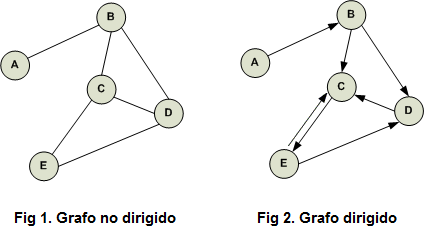
\includegraphics[scale=0.75]{grafos-dirigidos-y-no-dirigidos.png}
\end{center}
\end{frame}

\begin{frame}{\textquestiondown Para qué podemos usar los grafos?}
Mediante un grafo podemos representar, por ejemplo, una ciudad. Las esquinas serían los vértices y las conexiones por medio de una calle entre dos esquinas serían los ejes. Si todas las calles son doble mano, el grafo es no dirigido.
Si algunas calles son mano única el grafo es dirigido: ¿cómo modelamos una calle doble mano aquí?

\bigskip
A medida que los problemas se dificultan, puede suceder que sea difícil que a uno se le ocurra modelar el problema con un grafo, pero que una vez que lo hayamos hecho, el problema se vuelva sencillo utilizando los algoritmos que veremos hoy. 

\end{frame}

\begin{frame}
De ahora en más trabajaremos con grafos no dirigidos por simplicidad, pero también podrían aplicarse a grafos dirigidos.

\begin{block}{Vecindad}
Diremos que dos nodos son $adyacentes$ o $vecinos$ si existe una arista que los une.
\end{block}

\begin{block}{Distancia}
La distancia entre dos nodos $u$ y $v$ es la mínima cantidad de ejes por los que me tengo que mover para salir de $u$ y llegar a $v$. Si hay múltiples formas de llegar de $u$ a $v$, me quedo con la más corta.
\end{block}

\end{frame}

\begin{frame}{Formas de representar un grafo}
Existen varias maneras de guardar un grafo en memoria para poder luego consultar cosas (por ejemplo, recorrer el grafo, que es lo que haremos hoy).

Veamos las dos más populares.
\end{frame}

\begin{frame}{Matriz de adyacencia}
\begin{block}{Matriz de adyacencia}
La matriz de adyacencia es una matriz de $n \times n$ donde $n$ es la cantidad de nodos del grafo, que en la posición ($i,j$) tiene un 1 (o true) si hay una arista entre los nodos $i$ y $j$ y 0 (o false) si no.
\end{block}

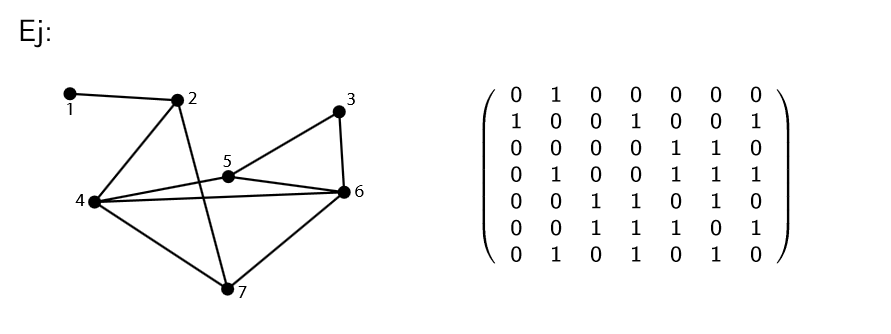
\includegraphics[scale=0.5]{matriz-adyacencia.png}
\end{frame}

\begin{frame}{Matriz de adyacencia}
Esta es una de las representaciones m\'as utilizadas. Si bien el ejemplo es para un grafo no dirigido, tambi\'en se puede utilizar la misma estructura para grafos dirigidos y grafos con pesos.
\bigskip

{\bf Ventajas}
\pause
\invisible<1> {
	\begin{itemize}
		\item Permite saber si existe o no arista entre dos nodos cualesquiera en O(1).
		\item Es muy f\'acil de implementar, $matrizAdy[i][j]$ guarda toda la informaci\'on sobre la arista.
	\end{itemize}
}
\bigpause
{\bf Desventajas}
\pause
\invisible<1> {
	\begin{itemize}
		\item La complejidad espacial: se necesitan $n^2$ casillas para representar un grafo de $n$ nodos.
	\end{itemize}
}
\end{frame}

\begin{frame}{Lista de adyacencia}
\begin{block}{Lista de adyacencia}
La lista de adyacencia es un vector de vectores de enteros, que en el $i$-ésimo vector tiene el número $j$ si hay una arista entre los nodos $i$ y $j$.
\end{block}

Coloquialmente la llamamos {\it lista de vecinos} pues para cada nodo guardamos la lista de nodos para los que existe una arista que los conecta (o sea, los vecinos).
\bigskip
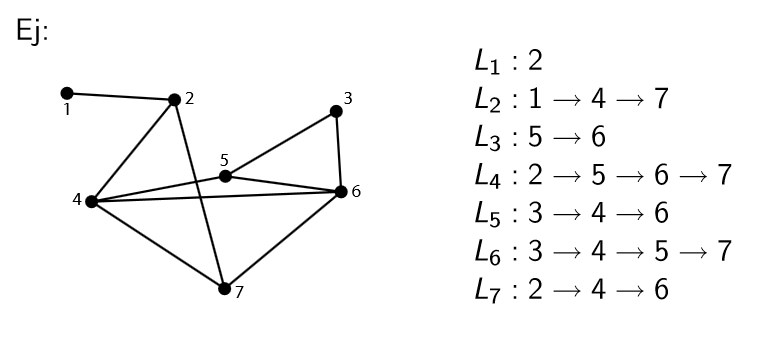
\includegraphics[scale=0.5]{lista-vecinos.png}
\end{frame}

\begin{frame}{Lista de adyacencia}
Nuevamente, con la misma idea tambi\'en se pueden modelar grafos dirigidos y con pesos.\bigskip

La complejidad espacial de esta representaci\'on ser\'a posiblemente mucho menor. ?`Cu\'anta memoria necesitaremos para un grafo de $n$ nodos y $m$ aristas? \pause {\bf O(m+n)}
\end{frame}


\section{Recorrer un grafo}
\begin{frame}{Recorrer un grafo}
A continuación vamos a ver dos algoritmos utilizados para recorrer grafos. Luego, podremos utilizar estos algoritmos para calcular lo que necesitemos (por ejemplo, distancias a un nodo en particular) o para encontrar un nodo en particular, que tenga una propiedad.

\bigskip
Ambos algoritmos tendrán una complejidad de $O(n+m)$, si $n$ es la cantidad de nodos y $m$ la de aristas, pero cada uno será útil en situaciones específicas.
\end{frame}


\begin{frame}{Una forma intuitiva de recorrer el grafo: DFS}
El DFS (Depth First Search) es un tipo de recorrido del grafo. Se dice que lo recorre \textit{en profundidad}, es decir, empieza por el nodo inicial y en cada paso visita un nodo vecino no visitado del nodo donde está parado, si no hay nodos por visitar vuelve para atrás.

\bigskip
Veamos un ejemplo visual de cómo se recorre un grafo con DFS.
\end{frame}


\begin{frame}{Ejemplo}
\tikzstyle{vertex}=[circle,fill=black!25,minimum size=20pt,inner sep=0pt]
\tikzstyle{selected vertex} = [vertex, fill=red!24]
\tikzstyle{edge} = [draw,thick,-]
\tikzstyle{weight} = [font=\small]
\tikzstyle{selected edge} = [draw,line width=5pt,-,red!50]
\tikzstyle{ignored edge} = [draw,line width=5pt,-,black!20]

\begin{figure}
\begin{tikzpicture}[scale=1.8, auto,swap]
    % Draw a 7,11 network
    % First we draw the vertices
    \foreach \pos/\name/\dist in {{(0,2)/0/0}, {(2,1)/1}, {(4,1)/2}, {(0,0)/3}, {(3,0)/4}, {(2,-1)/5}, {(4,-1)/6}}
        \node[vertex] (\name) at \pos {$\name$};
    % Connect vertices with edges and draw weights
    %\foreach \source/ \dest /\weight in {b/a/7, c/b/8,d/a/5,d/b/9,
           %                              e/b/7, e/c/5,e/d/15,
          %                               f/d/6,f/e/8,
         %                                g/e/9,g/f/11}
        %\path[edge] (\source) -- node[weight] {$\weight$} (\dest);
      \path[edge] (1) -- (0);
      \path[edge] (2) -- (1);
      \path[edge] (3) -- (0);
      \path[edge] (4) -- (3);
      \path[edge] (5) -- (3);
      \path[edge] (5) -- (4);
      \path[edge] (6) -- (5);
      
    \foreach \vertex / \fr in {0/1,1/2,2/3,3/4,5/5,4/6,6/7}
        \path<\fr-> node[selected vertex] at (\vertex) {$\vertex$};
    % For convenience we use a background layer to highlight edges
    % This way we don't have to worry about the highlighting covering
    % weight labels. 
    \begin{pgfonlayer}{background}
        \pause
        \foreach \source / \dest / \fr in {0/1/2,1/2/3,0/3/4,3/5/5,5/4/6,5/6/7}
            \path<\fr->[selected edge] (\source.center) -- (\dest.center);
    \end{pgfonlayer}
\end{tikzpicture}
\end{figure}
\end{frame}


\begin{frame}{Ejemplo}
En el ejemplo anterior vimos cómo recorre el grafo un DFS. Ahora tratemos de implementar un DFS resolviendo un problema (por supuesto, DFS se puede aplicar a muchos problemas más).

\begin{block}{Problema}
Dado un grafo conexo (es decir, que existe al menos un camino entre todo par de nodos) queremos ver si dicho grafo es un {\bf árbol}.
\end{block}

\textquestiondown Pero qué significa que un grafo sea un {\bf árbol}?
\end{frame}

\begin{frame}
\begin{block}{Árboles}
Un árbol es un tipo especial de grafo no dirigido. Es un grafo donde entre cualquier par de nodos existe un único camino que los conecta (notar que en particular, todos los nodos tienen que estar conectados entre sí).
\end{block}

Los árboles tienen mil propiedades interesantes, como $m = n -1$, que no tiene ciclos y más cosas sobre las que hoy no hablaremos.

%DIBUJITO
\end{frame}

\begin{frame}{Ideas para la resolución}
\begin{itemize}
\item Primero que nada, como tenemos un grafo vamos a querer recorrerlo y detectar si existe más de un camino entre algún par de nodos. ¿Pero cómo podemos hacer esto?
\pause
\invisible<1>{
\item Iremos recorriendo el grafo con DFS, siempre moviéndome a un vecino no visitado aún. Para no visitar un nodo dos veces (eso sería innecesario y empeoraría la performance) marcamos cada nodo cuando lo revisamos.  ¿Qué significa si llego a un nodo y un vecino de él (que no es por el que llegué) ya está visitado?}
\pause
\invisible<1-2>{
\item Significa que desde mi nodo inicial pude llegar a un nodo de dos formas distintas: es decir que no existe un único camino, lo que contradice la definición de árbol. Ergo, no es árbol. }
\end{itemize}
\end{frame}


%\pause
%\invisible<1>{
%\item Cuando llega a un nodo que ya fue visitado se da cuenta de que pudo acceder a ese nodo por dos caminos, eso %quiere decir que si recorremos uno de los caminos en un sentido y el otro camino en sentido opuesto formamos un ciclo.}
%\pause
%\invisible<1-2>{
%\item Asx como el BFS se implementa con una cola, el DFS se implementa con una pila.}
%\end{itemize}
%\end{frame}

\begin{frame}[fragile]{Pseudocódigo del DFS}
\begin{lstlisting}
// inicialmente se llena el vector visitado en false pues ningun nodo fue visitado
// ademas el nodo inicial no tiene padre y por eso se llama con padre = -1
bool esArbol(grafo, int nodoActual, vector<bool> &visitado, int padre):
    visitado[nodoActual] = true 

    para cada vecino v de nodoActual en grafo:
        si v ya fue visitado y v != padre:
            devolver false
            // encontre dos caminos distintos y luego no es arbol
        si v no fue visitado aun:
            si no esArbol(grafo, v, visitado, nodoActual): 
            // llamo recursivamente al dfs con el subarbol con raiz en v, ahora el padre es nodoActual
                devolver false
    
    // si para ningun vecino encontre algun ciclo, es un arbol porque se que es conexo
    devolver true
		
\end{lstlisting}
\end{frame}

\begin{frame}[fragile]{Implementación en C++ del DFS}
\begin{lstlisting}
bool esArbol(vector<vector<int> > &lista, int t, vector<bool> &visitado, int padre)
{
    visitado[t] = true;
    for(int i = 0; i < lista[t].size(); i++)
    {
        if(visitado[lista[t][i]] == true && lista[t][i] != padre)
            return false;
        if(visitado[lista[t][i]] == false)
            if(esArbol(lista, lista[t][i], visitado, t) == false)
                return false;
    }
    return true;
}
\end{lstlisting}
\end{frame}

\begin{frame}{Análisis del DFS}
\begin{itemize}
\item En ningún momento usamos una pila explícita, pero la pila está implícita en la recursión.
\pause
\invisible<1>{
\item Guardamos el padre del nodo, es decir, el nodo desde el cual fuimos a parar al nodo actual, para no confundir un ciclo con ir y volver por la misma arista.}
\pause
\invisible<1-2>{
\item Si el nodo ya lo visitamos y no es el nodo desde el cual venimos quiere decir que desde algún nodo llegamos por dos caminos, o sea que hay un ciclo.}
\pause
\invisible<1-3>{
\item Si el nodo no lo visitamos, pero desde uno de sus vecinos podemos llegar a un ciclo, entonces es porque hay un ciclo en el grafo y por lo tanto no es un árbol.}
\end{itemize}
\end{frame}

\begin{frame}{Otro algoritmo de búsqueda: BFS}
Muchas veces no basta con recorrer el grafo, sino que queremos hacerlo de una forma en particular. BFS suele ser muy útil en muchos problemas, veamos de qué se trata!
\bigskip

\begin{block}{Breadth First Search o \textit{búsqueda en anchura}}
El Breadth First Search o \textit{búsqueda en anchura} es un algoritmo que recorre un grafo comenzando por un nodo en particular, y se exploran todos los vecinos del nodo. Luego, se exploran todos los vecinos de los vecinos del nodo inicial, y así siguiendo hasta recorrer todos los nodos.
\end{block}

Veámoslo gráficamente.
\end{frame}

\begin{frame}{Ejemplo de recorrido de un grafo usando BFS}
\tikzstyle{vertex}=[circle,fill=black!25,minimum size=20pt,inner sep=0pt]
\tikzstyle{selected vertex} = [vertex, fill=red!24]
\tikzstyle{edge} = [draw,thick,-]
\tikzstyle{weight} = [font=\small]
\tikzstyle{selected edge} = [draw,line width=5pt,-,red!50]
\tikzstyle{ignored edge} = [draw,line width=5pt,-,black!20]

\begin{figure}
\begin{tikzpicture}[scale=1.8, auto,swap]
    % Draw a 7,11 network
    % First we draw the vertices
    \foreach \pos/\name/\dist in {{(0,2)/0/0}, {(2,1)/1}, {(4,1)/2}, {(0,0)/3}, {(3,0)/4}, {(2,-1)/5}, {(4,-1)/6}}
        \node[vertex] (\name) at \pos {$\name$};
    % Connect vertices with edges and draw weights
    %\foreach \source/ \dest /\weight in {b/a/7, c/b/8,d/a/5,d/b/9,
           %                              e/b/7, e/c/5,e/d/15,
          %                               f/d/6,f/e/8,
         %                                g/e/9,g/f/11}
        %\path[edge] (\source) -- node[weight] {$\weight$} (\dest);
      \path[edge] (1) -- (0);
      \path[edge] (2) -- (1);
      \path[edge] (3) -- (0);
      \path[edge] (4) -- (3);
      \path[edge] (5) -- (3);
      \path[edge] (5) -- (4);
      \path[edge] (6) -- (5);
      
    \foreach \vertex / \fr in {0/1,1/2,3/3,2/4,4/5,5/6,6/7}
        \path<\fr-> node[selected vertex] at (\vertex) {$\vertex$};
    % For convenience we use a background layer to highlight edges
    % This way we don't have to worry about the highlighting covering
    % weight labels. 
    \begin{pgfonlayer}{background}
        \pause
        \foreach \source / \dest / \fr in {0/1/2,0/3/3,1/2/4,3/4/5,3/5/6,5/6/7}
            \path<\fr->[selected edge] (\source.center) -- (\dest.center);
    \end{pgfonlayer}
\end{tikzpicture}
\end{figure}
\end{frame}


\begin{frame}
Implementemos un BFS resolviendo un problema. Vale notar que este problema no podía ser resuelto con DFS.

\begin{block}{Calcular las distancias de un nodo a todos los demás}
Dado un nodo inicial, queremos hallar la distancia de cada nodo a todos los demás. Recordemos que puede haber más de una forma de ir de un nodo a otro, pero para la distancia siempre tomaremos la mínima.
\end{block}

\textquestiondown Cómo podemos resolverlo usando BFS? Por ahora no nos centremos en cómo se implementa el algoritmo, sino en cómo usarlo para resolver el problema. Luego intentaremos implementarlo.
\end{frame}

\begin{frame}{Detalles de implementación del BFS}
\begin{itemize}
\item Las distancias del nodo inicial a los demás nodos las inicializaremos en infinito (en principio no sabemos a qué distancia están, luego iremos actualizando el valor si encontramos un camino desde el nodo inicial al nodo).
\pause
\invisible<1>{
\item Usaremos una cola para ir agregando los nodos por visitar. Como agregamos primero todos los vecinos del nodo inicial, los primeros nodos en entrar a la cola son los de distancia 1, luego agregamos los vecinos de esos nodos, que son los de distancia 2, y así vamos recorriendo el grafo en orden de distancia al vértice inicial.}
\pause
\invisible<1-2>{
\item Cuando visitamos un nodo, sabemos cuáles de sus vecinos agregar a la cola. Tenemos que visitar los vecinos que todavía no han sido visitados.}
\end{itemize}
\end{frame}

\begin{frame}[fragile]{Pseudoc\'odigo del BFS}

\begin{lstlisting}
vector<int> BFS (Grafo listaAdyacencias, int nodoInicial):
   cantidadDeNodos = longitud(listaAdyacencias)
   queue<int> cola // aqui encolare los nodos que todavia no analizamos

   // distancias[i] = distancia de i a nodoInicial, inicialmente es INFINITO
   vector<int> distancias(cantidadDeNodos, INFINITO) 

   cola.encolar(nodoInicial)
   distancias[nodoInicial] = 0
   mientras (la cola no esta vacia):
       tope = cola.tope() // tomo el tope de la cola (y lo saco de la cola)

       para todos los vecinos v de "tope" en el grafo:
           si la distancia entre v y el nodoInicial es infinito:
               distancias[v] = distancias[tope] + 1 // esta un nodo mas lejos que su vecino
               cola.encolar(v) // encolo v para analizarlo luego

   devolver distancias
\end{lstlisting}
\end{frame}


\begin{frame}[fragile]{Implementaci\'on del BFS}
\begin{lstlisting}
vector<int> BFS(vector<vector<int> > &lista, int nodoInicial){
    int n = lista.size(),t;
    queue<int> cola;
    vector<int> distancias(n,n);
    cola.push(nodoInicial);
    distancias[nodoInicial] = 0;
    while(!cola.empty()){
        t = cola.front();
        cola.pop();
        for(int i=0;i<lista[t].size();i++){
            if(distancias[lista[t][i]]==n){
                distancias[lista[t][i]] = distancias[t]+1;
                cola.push(lista[t][i]);
            }
        }
    }
    return distancias;
}
\end{lstlisting}
\end{frame}


\begin{frame}
\begin{center}
{\Huge \textquestiondown Preguntas?}
\end{center}
\end{frame}

\end{document}
